\documentclass{beamer}

\usepackage[utf8]{inputenc}
\usepackage{amsmath}
\usepackage{graphicx}
\usepackage{xcolor}
\usepackage{style}
\usepackage[ddmmyyyy]{datetime}
\usepackage{tabstackengine}
\usepackage{amsmath}
\usepackage{svg}

\title{Kalman Filter}
\subtitle{Grundlagen}
\author{P.~Schön (5121059), C.~Thein (5121017)}
\date{\today}
\renewcommand{\dateseparator}{.}
\newcommand\w[1]{\makebox[2.5em]{$#1$}}
\addtobeamertemplate{footnote}{\hspace{25ex}}{}

\setbeamertemplate{sections/subsections in toc}[square]
% \setbeamertemplate{sections/subsections in toc}[sections numbered]
% \setbeamertemplate{caption}[numbered]

\usefonttheme[onlymath]{serif}

\begin{document}

\frame{\titlepage}

\begin{frame}
    \frametitle{Table of contents}
    \begin{columns}
        \begin{column}{0.4\textwidth}
            \tableofcontents
        \end{column}
        \begin{column}{0.4\textwidth}
            \begin{figure}
                \centering
                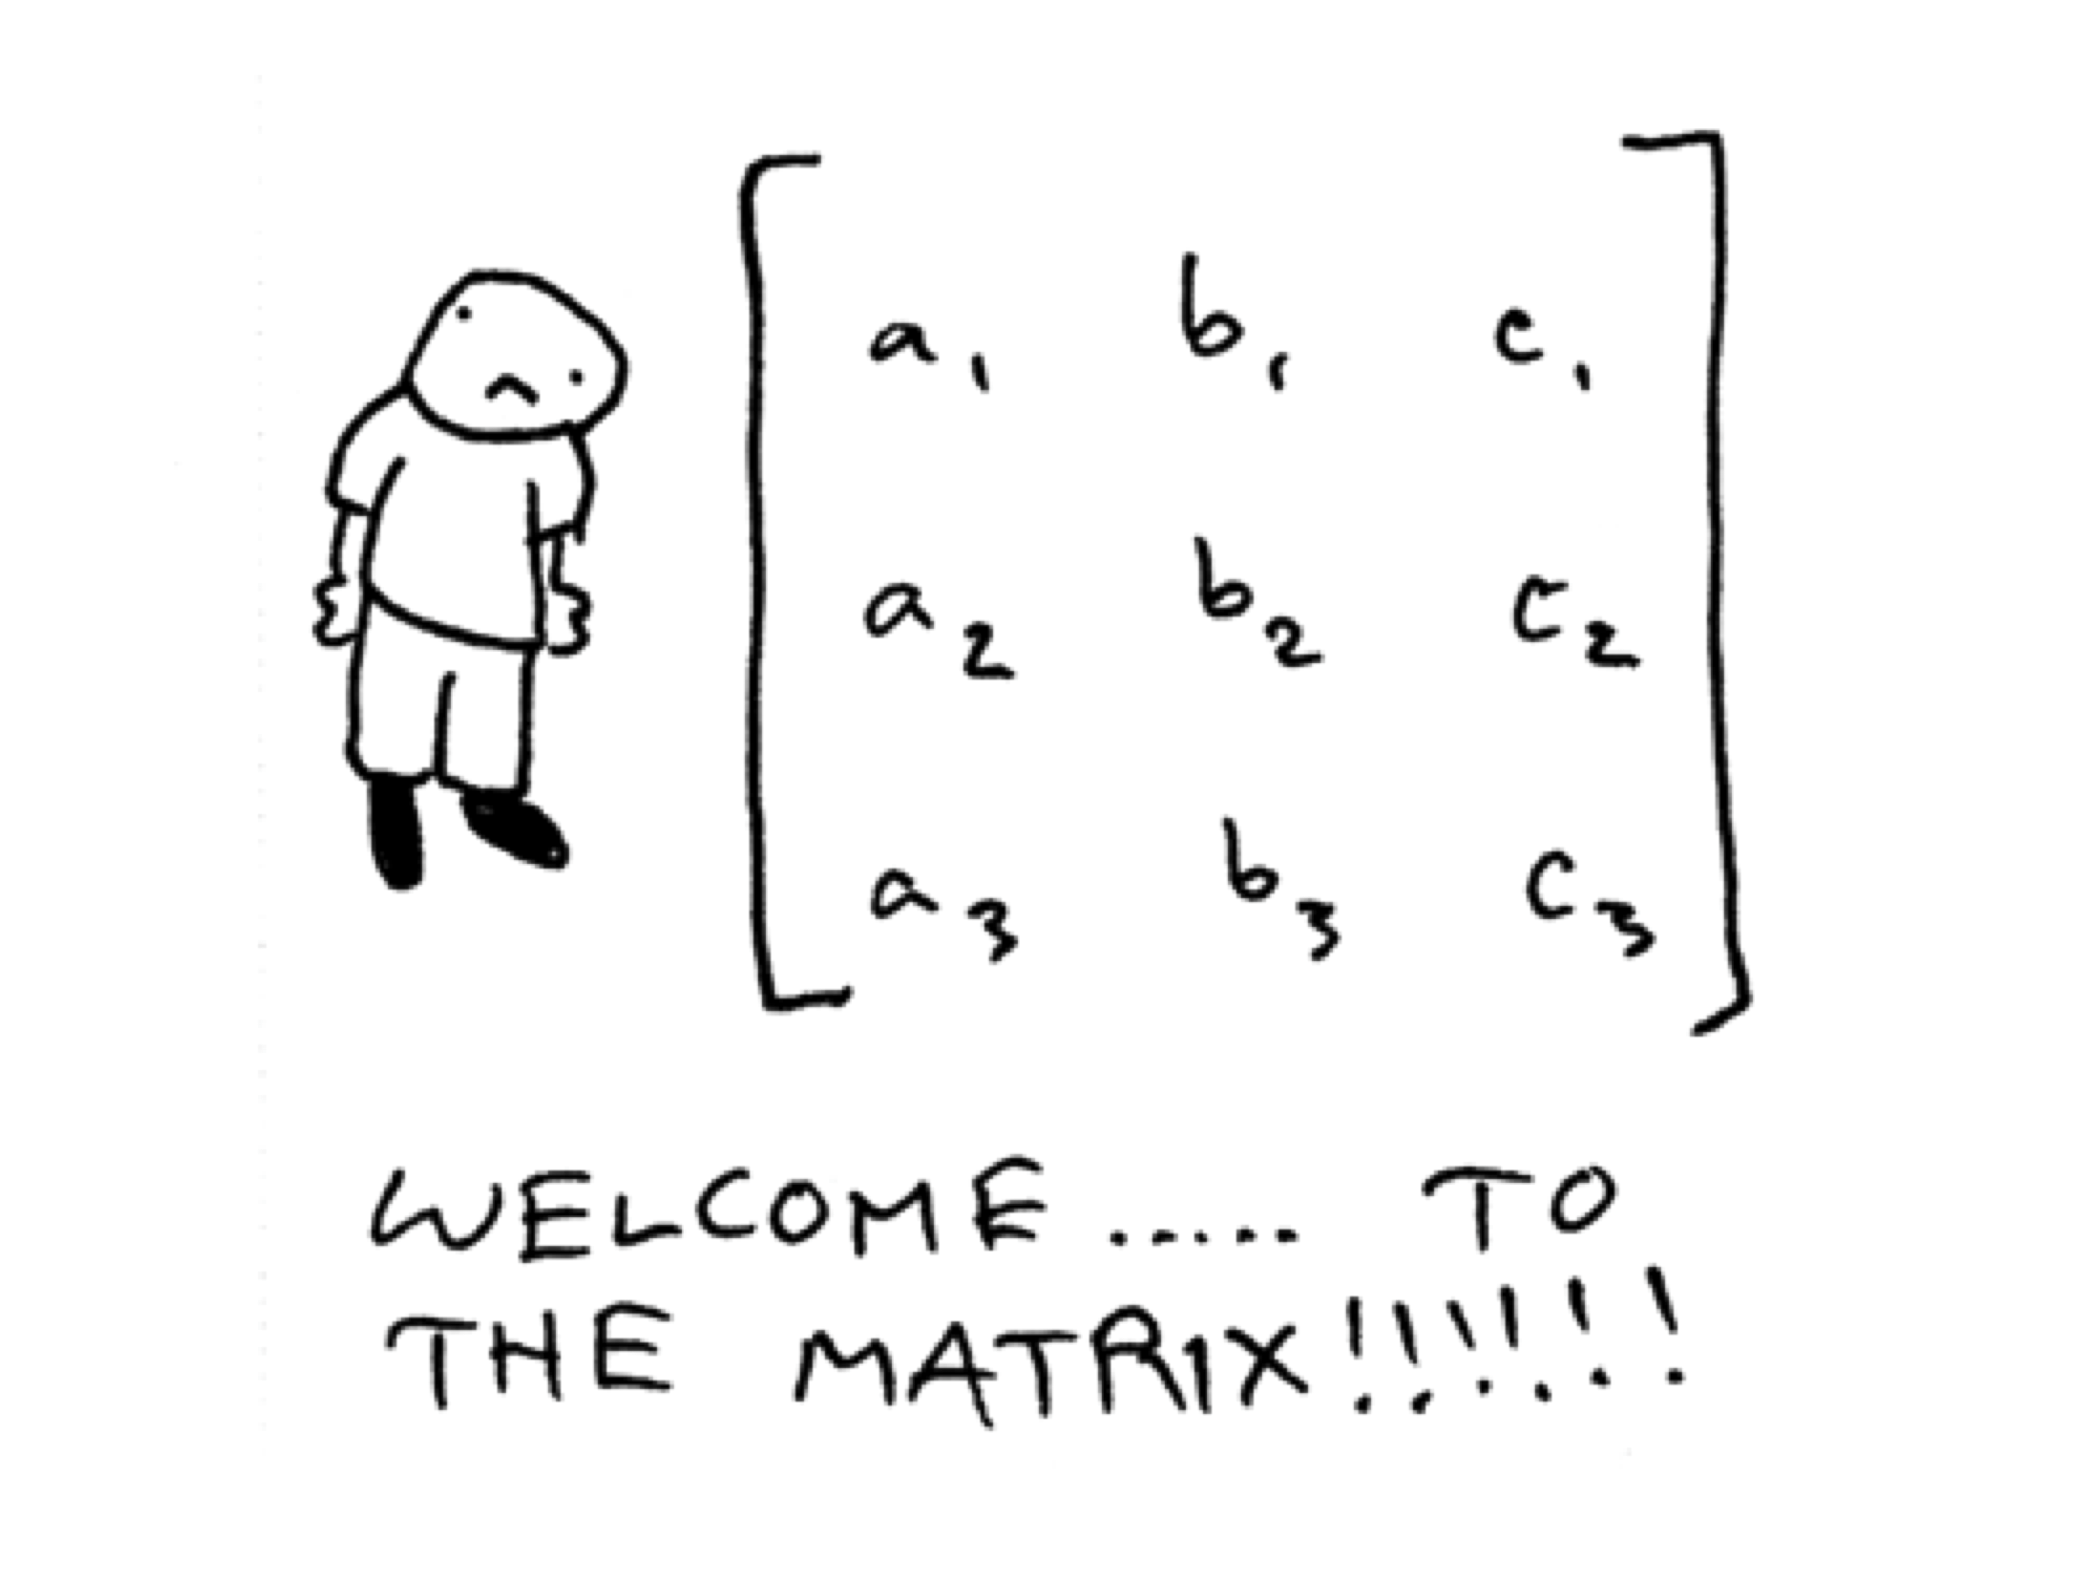
\includegraphics[width=1\textwidth]{images/graphics/Bildschirmfoto 2024-06-02 um 16.40.09.png}
            \end{figure} 
        \end{column}
    \end{columns}
\end{frame}

\section{Introduction}

% ABOUT KALMAN BOY
\begin{frame}
    \frametitle{Rudolf Emil Kalman}
    \begin{columns}
        \begin{column}{0.7\textwidth}
           \begin{itemize}
            \item was born in 1930 in Hungary
            \item Bachelor of Science and Master of Science at the MIT
            \item PHD 1957 at the Columbia
            \item developed the filter arond the years 1960 to 1961
            \item died in 2016 in Florida
           \end{itemize} 
        \end{column}
        \begin{column}{0.3\textwidth}
            \begin{figure}
                \centering
                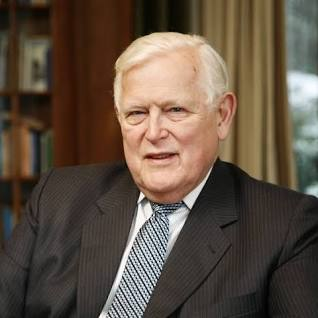
\includegraphics[width=1\textwidth]{images/graphics/kalman_bre.jpeg}
                \caption{Rudolf Emil Kalman}
            \end{figure}
        \end{column}
    \end{columns}
\end{frame}

% KALMAN FILTER FIRST EXPLAINATION
\begin{frame}
    \frametitle{What is the Kalman Filter?}
    The Kalman filter is a mathematical method for iteratively estimating parameters to describe
    system states.

    In this process, a prediction about a parameter value is repeatedly made, combined with the
    error-prone measurement, and then used again to make a new prediction.
\end{frame}

% KALMAN FILTER PROCESS GRAPHIC
\begin{frame}
    \frametitle{Kalman Filter}
    \begin{figure}
        \centering
        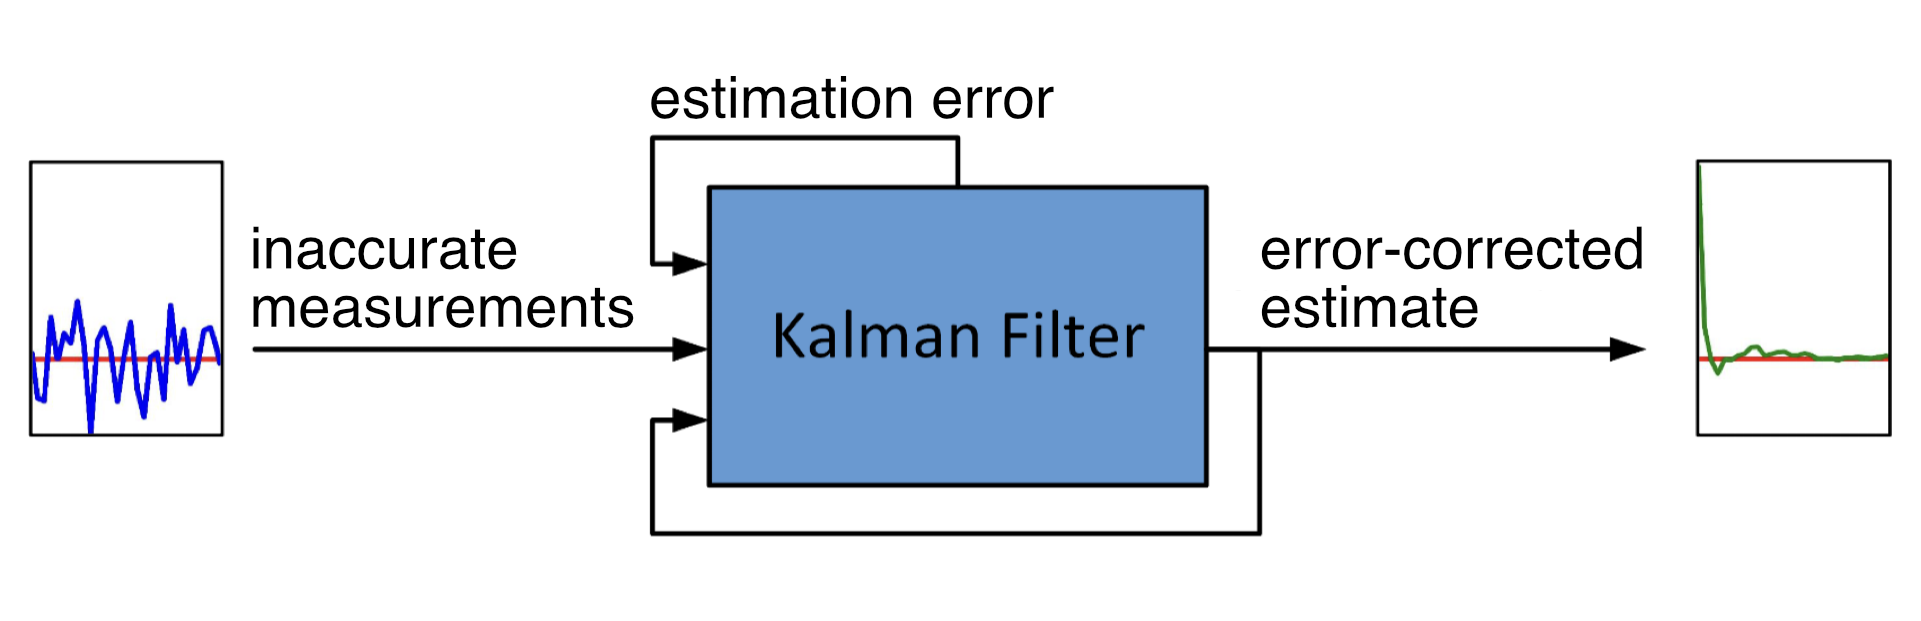
\includegraphics[width=1\textwidth]{images/graphics/flow.png}
        \caption{Procedure of the Kalman Filter\footnotemark}
    \end{figure}
\end{frame}

% APPLICATION EXAMPLE
% TODO: Add some Esy to follow real world example here.

% LIST OF SENSOR EXAMPLES
\begin{frame}
    \frametitle{Sensors susceptible to failure}
    \begin{columns}

        \begin{column}{0.4\textwidth}
            \footnotesize
            \begin{itemize}
                \item Light sensor (photoresistor)
                \item Ultrasonic sensor
                \item Infrared sensor
                \item Temperature sensor (thermoelectric)
                \item Magnetic field sensor
                \item Gas and air quality sensor
                \item Humidity sensor
                \item Motion sensor (accelerometer)
                \item Pressure sensor
                \item Sound sensor
            \end{itemize}
        \end{column}
        
        \begin{column}{0.6\textwidth}
            \begin{figure}
                \centering
                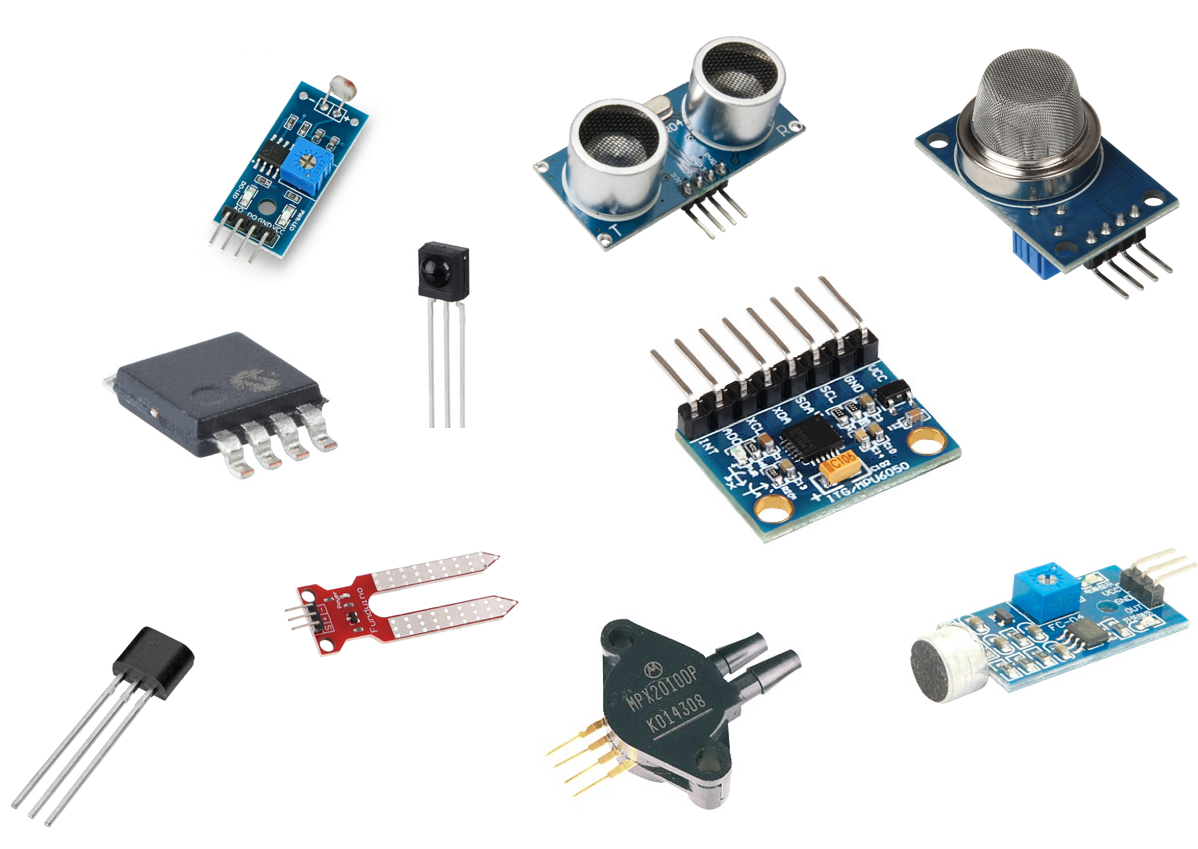
\includegraphics[width=1\textwidth]{images/graphics/sensors.png}
                \caption{sensors}
            \end{figure}
        \end{column}

    \end{columns}
\end{frame}

\section{Foundations}

% FIRST STATISTICAL FOUNDATIONS
% THE MEAN VALUE
\begin{frame}
    \frametitle{The Mean}
    \begin{figure}
        \centering
        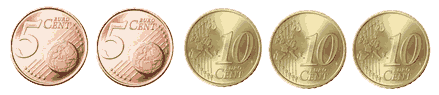
\includegraphics[width=1\textwidth]{images/graphics/coins.png}
    \end{figure}
    \vspace{1cm}
    \begin{equation*}
        \mu = \frac{1}{N} \sum _{n=1}^{N}V_{n}= \frac{1}{5} \left( 5+5+10+10+10 \right) = 8 \text{ Cent}
    \end{equation*}
\end{frame}

% THE STANDARD DEVIATION
\begin{frame}
    \frametitle{The standarddeviation}


    \footnotesize
    \begin{tabular}{ c|ccccc|c }
        \hline
             & Player1 & Player2 & Player3 & Player4 & Player5 & Mean \\ 
        \hline
            Team A & \(1.89\)m & \(2.10\)m & \(1.75\)m & \(1.98\)m & \(1.85\)m & \(1.914\)m \\ 
            Team B & \(1.94\)m & \(1.90\)m & \(1.97\)m & \(1.89\)m & \(1.87\)m & \(1.194\)m \\ 
        \hline
    \end{tabular}

    \vspace{0.5cm}

    \normalsize
    \begin{equation*}
        x_{n} -  \mu = x_{n}-1.914m
    \end{equation*}

    \vspace{0.5cm}

    \footnotesize
    \begin{tabular}{ c|ccccc }
        \hline
             & Player1 & Player2 & Player3 & Player4 & Player5 \\ 
        \hline
            Team A & \(-0.024\)m & \(0.186\)m & \(-0.164\)m & \(0.066\)m & \(-0.064\)m \\ 
            Team B & \(0.026\)m & \(-0.014\)m & \(0.056\)m & \(-0.024\)m & \(-0.044\)m \\ 
        \hline
    \end{tabular}


\end{frame}

% THE VARIANCE I
\begin{frame}
    \frametitle{The variance}

    \footnotesize
    % \scriptsize
    \begin{tabular}{ c|ccccc }
        \hline
             & Player1 & Player2 & Player3 & Player4 & Player5 \\ 
        \hline
            Team A & \(-0.024\)m & \(0.186\)m & \(-0.164\)m & \(0.066\)m & \(-0.064\)m \\ 
            Team B & \(0.026\)m & \(-0.014\)m & \(0.056\)m & \(-0.024\)m & \(-0.044\)m \\ 
        \hline
    \end{tabular}

    \vspace{0.5cm}

    \normalsize
    \begin{equation*}
        \left( x_{n}-  \mu  \right) ^{2} =  \left( x_{n}- 1.914m \right) ^{2}
    \end{equation*}

    \vspace{0.5cm}

    \tiny
    \begin{tabular}{ c|ccccc }
        \hline
             & Player1 & Player2 & Player3 & Player4 & Player5 \\ 
        \hline
            Team A & \(0.000576\)m\(^{2}\) & \(0.034596\)m\(^{2}\) & \(0.026896\)m\(^{2}\) & \(0.004356\)m\(^{2}\) & \(0.004096\)m\(^{2}\) \\ 
            Team B & \(0.000676\)m\(^{2}\) & \(0.000196\)m\(^{2}\) & \(0.003136\)m\(^{2}\) & \(0.000576\)m\(^{2}\) & \(0.001936\)m\(^{2}\) \\ 
        \hline
    \end{tabular}

\end{frame}

% THE VARIANCE II
\begin{frame}
    \frametitle{The variance}
    
    \begin{equation*}
        \sigma^{2} = \frac{1}{N} \sum _{n=1}^{N} \left( x_{\scriptscriptstyle \!B_{n}} -  \mu  \right) ^{2}
    \end{equation*}

    \vspace{5mm}
    \tiny
    \begin{equation*}
        \sigma_{\scriptscriptstyle \!A}^{2} = \frac{1}{N} \sum _{n=1}^{N} \left( x_{\scriptscriptstyle \!A_{n}} -  \mu  \right) ^{2} = \frac{1}{5} \left( 0.000576+ 0.034596+ 0.026896+ 0.004356+ 0.004096 \right) = 0.014m^{2}
    \end{equation*}
    
    \vspace{1mm}
    
    \begin{equation*}
       \sigma_{\scriptscriptstyle \!B}^{2} = \frac{1}{N} \sum _{n=1}^{N} \left( x_{\scriptscriptstyle \!B_{n}} -  \mu  \right) ^{2} = \frac{1}{5} \left( 0.000676+ 0.000196+ 0.003136+ 0.000576+ 0.001936 \right) = 0.0013m^{2}
    \end{equation*}
   
\end{frame}

% THE COVARIANCE
\begin{frame}
    \frametitle{Covariance}
    \footnotesize

    \begin{itemize}
        \item \textbf{Definition:}
        Covariance is a measure of how much two random variables change together. If the greater values of one variable mainly correspond with the greater values of the other variable, and the same holds for the lesser values (i.e., the variables tend to show similar behavior), the covariance is positive. In the opposite case, when the greater values of one variable mainly correspond to the lesser values of the other (i.e., the variables tend to show opposite behavior), the covariance is negative.
    \end{itemize}

    \begin{block}{Mathematical Definition}
        Given two random variables \(X\) and \(Y\), the covariance is defined as:
        \[
        \text{Cov}(X, Y) = \mathbb{E}[(X - \mathbb{E}[X])(Y - \mathbb{E}[Y])]
        \]
        where \(\mathbb{E}[X]\) and \(\mathbb{E}[Y]\) are the expected values (means) of \(X\) and \(Y\), respectively.
    \end{block}
\end{frame}

% THE COVARIANCE, TOO
\begin{frame}
    \frametitle{The covariance}
    \begin{itemize}
        \item \textbf{Example:}
        Consider two random variables, \(X\) and \(Y\), representing the number of hours studied and the test scores of students. If higher hours of study tend to correspond with higher test scores, the covariance between \(X\) and \(Y\) would be positive.
    \end{itemize}

    \begin{block}{Properties}
        \begin{itemize}
            \item \(\text{Cov}(X, Y) = \text{Cov}(Y, X)\)
            \item \(\text{Cov}(X, X) = \text{Var}(X)\) (Variance of \(X\))
            \item If \(X\) and \(Y\) are independent, \(\text{Cov}(X, Y) = 0\)
        \end{itemize}
    \end{block}

\end{frame}

\section{Simplified explanation}

% PROCESS EQUATIONS FOR THE KALMAN FILTER
\begin{frame}
    \frametitle{Process of Kalman Filters}

    \textbf{Prediction}

    1. State prediction: \( \hat{x}_{k} = A\hat{x}_{k-1}+Bu_{k-1} \)

    2. Covariance prediction: \( P_{k}=AP_{k-1}A^{T}+Q \)

    \textbf{Correction}

    3. Kalman Gain Prediction: \( K_{k}=P_{k}H^{T}(HP_{k}H^T+R)^{-1} \)

    4. State Update: \( \hat{x}_{k}=\hat{x}_{k}+K_{k}(z_{k}-H\hat{x}_{k}) \)

    5. Covariance Update: \( P_{k}=(I-K_{k}H)P_{k} \)
\end{frame}

% KALMAN EXAMPLE WITH THE GAUSS STUFF
\begin{frame}
    \frametitle{Kalman explained}
    \begin{figure}
        \centering
        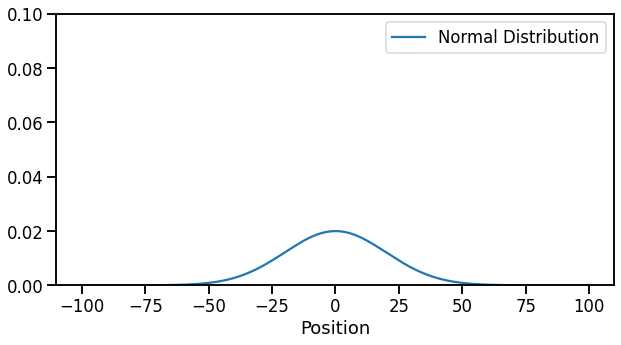
\includegraphics[width=0.7\textwidth]{images/01_normal_distribution.png}
        \caption{Start Postion at \(t_0\)}
    \end{figure}
\end{frame}

% KALMAN EXAMPLE WITH THE GAUSS STUFF
\begin{frame}
    \frametitle{Kalman explained}
    \begin{figure}
        \centering
        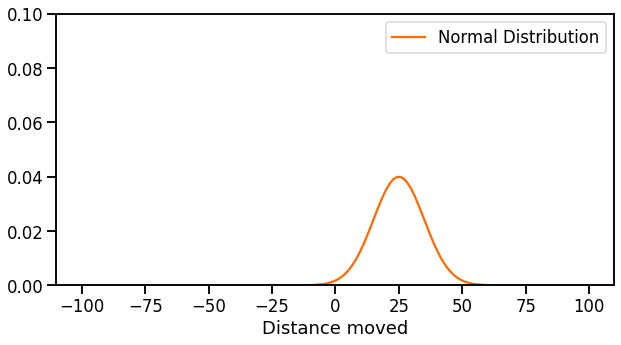
\includegraphics[width=0.9\textwidth]{images/02_normal_distribution_after_move.png}
        \caption{Calculated Postion at \(t_1\)}
    \end{figure}
\end{frame}

% KALMAN EXAMPLE WITH THE GAUSS STUFF
\begin{frame}
    \frametitle{Kalman explained}
    \begin{figure}
        \centering
        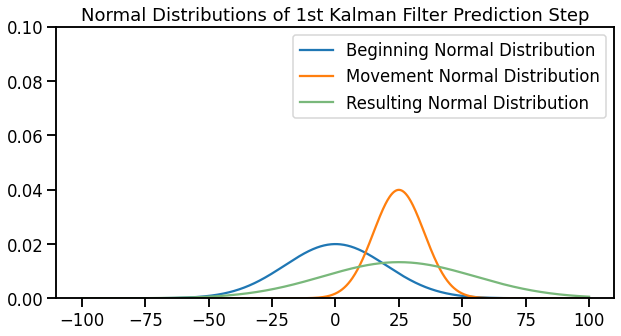
\includegraphics[width=0.9\textwidth]{images/03_first_prediction.png}
        \caption{Predicted Postion at \(t_1\)}
    \end{figure}
\end{frame}

% KALMAN EXAMPLE WITH THE GAUSS STUFF
\begin{frame}
    \frametitle{Kalman explained}
    \begin{figure}
        \centering
        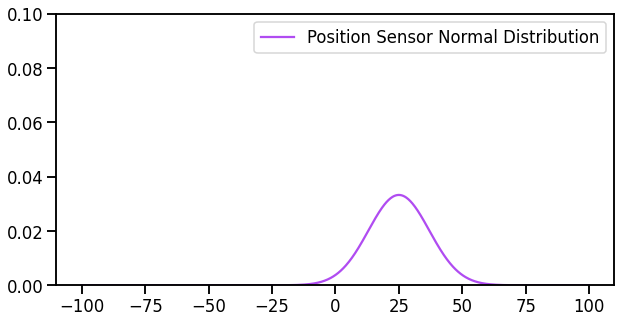
\includegraphics[width=0.9\textwidth]{images/04_measurement.png}
        \caption{Messured Sensor Data of Postion at \(t_1\)}
    \end{figure}
\end{frame}

% KALMAN EXAMPLE WITH THE GAUSS STUFF
\begin{frame}
    \frametitle{Kalman explained}
    \begin{figure}
        \centering
        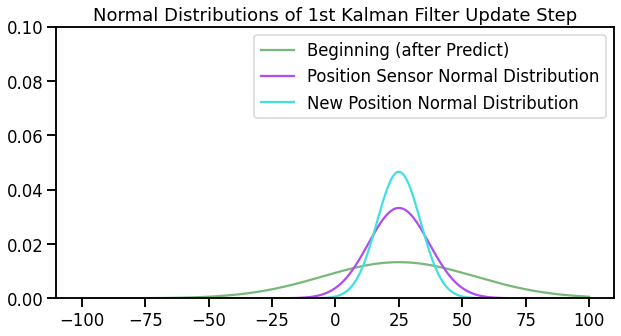
\includegraphics[width=0.9\textwidth]{images/05_correction.png}
        \caption{Correction of the Kalman Gain after measurement at \(t_1\)}
    \end{figure}
\end{frame}

% KALMAN EXAMPLE WITH THE GAUSS STUFF
\begin{frame}
    \frametitle{Takeaways}
    \begin{itemize}
        \item The precision decreases with the prediction
        \item The precision increases with the correction
    \end{itemize}

\end{frame}

\section{Joystick example}

\begin{frame}
    % TODO: Make Section Header Files
    \huge
    \textbf{Einbindung in einen konkreten Anwendungsfall}
\end{frame}

\begin{frame}
    \frametitle{State Representation}
    % //TODO: Make x's differentiabable
    We define the state vector \(x\) to include the position and velocity of the mouse in both x and y directions

    \begin{equation*}
        x = \begin{bmatrix}
            x     \\
            y     \\
            v_{x} \\
            v_{y} \\
        \end{bmatrix}
    \end{equation*}

    where:
    \begin{itemize}
        \item \(x\) is the position on the x-axis
        \item \(y\) is the postion on the y-axis
        \item \(v_{x}\) is the velocity in the x-direction
        \item \(v_{y}\) is the velocity in the y-direction

    \end{itemize}
\end{frame}

\begin{frame}
    \frametitle{Formulate the Transtition Model}
    The state transition model describes how the state evolves from one time step to the next.
    If we assume a constant velocity model, the state transition can be expressed as:
    \begin{equation*}
        x_{k+1}=Ax_{k}+w_{k}
    \end{equation*}
    where \(w_{k}\) represents the proces noise, assumed to be Gaussian with zero mean and covariance \(Q\).
\end{frame}

\begin{frame}
    \frametitle{Create the Transition Matrix}
    The transition matrix A for a constant velocity Model is:

    \begin{equation*}
        A = \begin{bmatrix}
            1 & 0 & \Delta t & 0        \\
            0 & 1 & 0        & \Delta t \\
            0 & 0 & 1        & 0        \\
            0 & 0 & 0        & 1        \\
        \end{bmatrix}
    \end{equation*}

    \(\Delta t\) is the time intervall between mesurements.
\end{frame}

\begin{frame}
    \frametitle{Observation Model}
    The observation model realtes the state to the measurements:
    \begin{equation*}
        z_{k}=Hx_{k}+v_{k}
    \end{equation*}
    where \(v_{k}\) represents the measurement noise, assumed to be Gaussian with zero mean and
    covariance \(R\).

    The observation matrix \(H\) for direct measurement of position is:

    \begin{equation*}
        H = \begin{bmatrix}
            1 & 0 & 0 & 0 \\
            0 & 1 & 0 & 0 \\
        \end{bmatrix}
    \end{equation*}

\end{frame}

\begin{frame}
    \frametitle{Prediction Step}

    The prediction step estimates the next state and its uncertainty:

    \begin{itemize}
        \item Predict the state:
              \begin{equation}
                  x_{k+1}=Ax_{k}
              \end{equation}

        \item Predict the error coavriance:
              \begin{equation}
                  P_{k+1}=AP_{k}A^{T}+Q
              \end{equation}
    \end{itemize}
\end{frame}

\begin{frame}
    \frametitle{Correction Step}
    The correction step updates the state estimate with the new measurement:
    \begin{itemize}
        \item Compute the Kalman gain:
              \begin{equation}
                  K_{k} = P_{k}H^{T}(HP_{k}H^{T}+R)^{-1}
              \end{equation}
        \item Update the state estimate:
              \begin{equation}
                  x_{k} = x_{k}+K_{k}(z_{k}-Hx_{k})
              \end{equation}
        \item Update the error covariance:
              \begin{equation}
                  P_{k} = (I-K_{k}H)P_{k}
              \end{equation}
    \end{itemize}
\end{frame}

\begin{frame}
    \frametitle{Kalman Filter}
    \begin{figure}
        \centering
        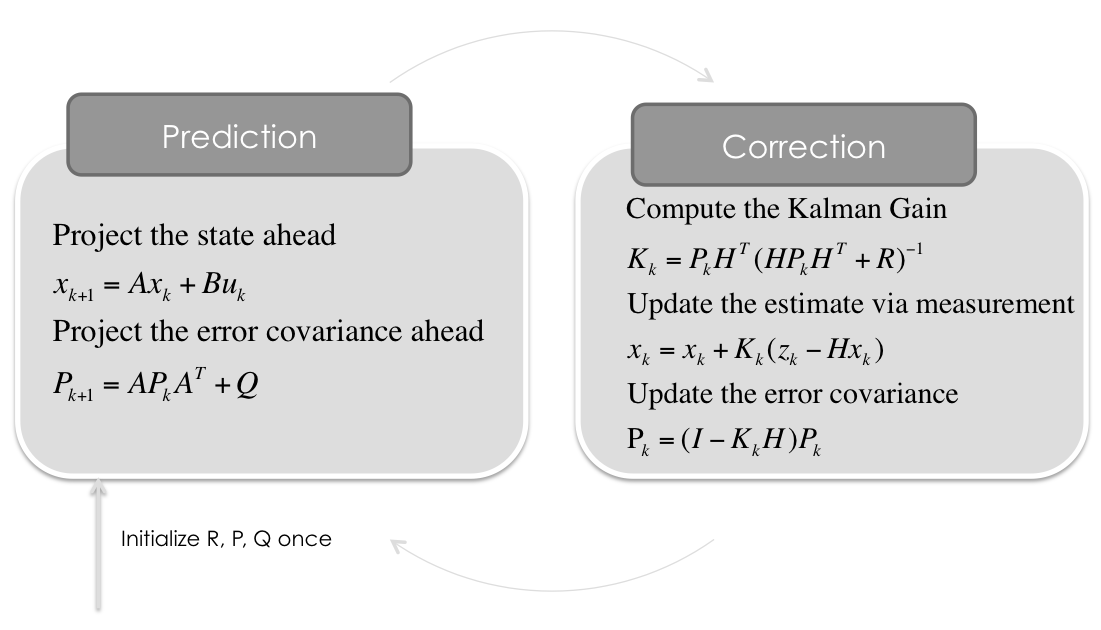
\includegraphics[width=0.95\textwidth]{images/06_kalman_diagram.png}
        \caption{Iterative Nature of the Kalman filter}
    \end{figure}
\end{frame}

\begin{frame}
    \frametitle{Cheat Sheet - Math Symbols}
    \scriptsize
    \begin{table}[h]
        \centering
        \begin{tabular}{|c|p{8cm}|}
            \hline
            \textbf{Symbol} & \textbf{Meaning}                                                                                                                                  \\ \hline
            \(k\)           & Interval or iteration of the Kalman filter                                                                                                        \\ \hline
            \(z_k\)         & Measurement vector. This contains the real-world measurement we received in this time step.                                                       \\ \hline
            \(x_k\)         & Newest estimate of the current "true" state.                                                                                                      \\ \hline
            \(P_k\)         & Newest estimate of the average error for each part of the state.                                                                                  \\ \hline
            \(R\)           & Estimated measurement error covariance. Finding precise values for Q and R are beyond the scope of this guide.                                    \\ \hline
            \(Q\)           & Estimated process error covariance. Finding precise values for Q and R are beyond the scope of this guide.                                        \\ \hline
            \(A\)           & State transition matrix. Basically, multiply state by this and add control factors, and you get a prediction of the state for the next time step. \\ \hline
            \(H\)           & Observation matrix. Multiply a state vector by H to translate it to a measurement vector.                                                         \\ \hline
            \(B\)           & Control matrix. This is used to define linear equations for any control factors.                                                                  \\ \hline
            \(u_{k-1}\)     & Control vector. This indicates the magnitude of any control system's or user's control on the situation.                                          \\ \hline
        \end{tabular}
    \end{table}
\end{frame}

\section{Summary}

\begin{frame}
    \frametitle{Summary}
    KALMA KALMA !
    
    \huge TO TH MOOOOOON!
\end{frame}

\begin{frame}
    \frametitle{List of figures}
    \listoffigures
    \footnotetext[1]{A test footnote in the first column}
\end{frame}

\end{document}
\ProvidesPackage{beamerthemesss}
\mode<presentation>
\usepackage{xcolor}
\usepackage{tikz}
\RequirePackage{enumitem} 


\definecolor{orange_100}{RGB}{255, 107, 0} 	% orange_100
\definecolor{orange_80}{RGB}{255, 137, 51} 	% orange_80
\definecolor{black_100}{RGB}{0, 0, 0} 		% black_100
\definecolor{black_80}{RGB}{50, 50, 50} 		% black_80
\definecolor{black_60}{RGB}{100, 100, 100} 	% black_60
\definecolor{white}{RGB}{255, 255, 255} 		% white


% Define a command to set the foreground color of lists
\newcommand{\setlistcolor}[1]{
    \setlist[enumerate]{label=\textcolor{#1}{\textbullet}}
    \setlist[itemize]{label=\textcolor{#1}{\textbullet}}
}
\setlistcolor{orange_80}

% Schriftarten einstellen
\setbeamerfont{title}{size=\huge,series=\bfseries}
\setbeamerfont{subtitle}{size=\small,series=\bfseries}
\setbeamerfont{frametitle}{size=\large,series=\bfseries}
\setbeamerfont{normal text}{size=\small}

% Farben anwenden
\setbeamercolor{title}{fg=orange_100}
\setbeamercolor{subtitle}{fg=black_60}
\setbeamercolor{frametitle}{fg=orange_100}
\setbeamercolor{section in toc}{fg=black_80}
\setbeamercolor{normal text}{fg=black_80}
\renewcommand{\figurename}{\textcolor{orange_100}{Fig.}}

% Layout anpassen
\setbeamertemplate{navigation symbols}{}

% Customize header and footer with dotted lines made of circles
\setbeamertemplate{headline}{
    \begin{tikzpicture}[remember picture,overlay]
    	\ifnum\theframenumber=1
        \node[anchor=north east, inner sep=0pt, yshift=-0.5mm, xshift=-2mm] at (current page.north east) {
            
\includegraphics[height=4.8mm]{logo.png}
        };
        \fi
        \draw[thick, dash pattern=on 0pt off 2\pgflinewidth, line cap=round, color=orange_100]
              ([yshift=-7.5mm]current page.north west) -- 
              ([yshift=-7.5mm]current page.north east);
    \end{tikzpicture}
}

\setbeamertemplate{footline}{
    \begin{tikzpicture}[remember picture,overlay]
        \ifnum\theframenumber>1
        	\draw[thick, dash pattern=on 0pt off 2\pgflinewidth, line cap=round, color=orange_100] 
              ([yshift=8mm]current page.south west) -- 
              ([yshift=8mm]current page.south east);
                      \node[anchor=east, inner sep=0pt, yshift=2.5mm, xshift=-5mm] at (current page.south east) {
        					\color{black_60}
        					\insertframenumber/
        					\inserttotalframenumber
        	};
        	\node[anchor=west, inner sep=0pt, yshift=3.5mm, xshift=-2mm] at (current page.south west) {
        		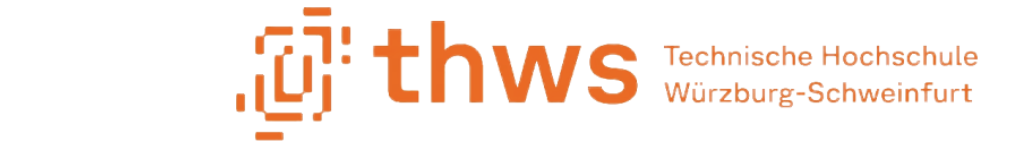
\includegraphics[height=7.8mm]{watermark.png}
        	};
        \fi
        \ifnum\theframenumber=1
        	\node[anchor=west, inner sep=0pt, yshift=6mm, xshift=-4mm] at (current page.south west) {
        		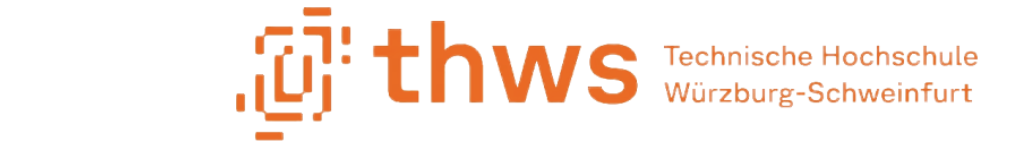
\includegraphics[height=9.8mm]{watermark.png}
        	};
        \fi

    \end{tikzpicture}
}

% Abschnittsüberschriften
\setbeamercolor{section in head/foot}{bg=orange_100,fg=white}
\setbeamerfont{section in head/foot}{series=\bfseries}
\setbeamertemplate{section in head/foot shaded}{\color{orange_100!50}}

\setbeamertemplate{frametitle}{
    \begin{tikzpicture}[remember picture,overlay]
        \node[
        	anchor=base west, 
        	fill=white, 
        	yshift=-3.9mm, 
        	xshift=-2mm
        ] {\bfseries\insertframetitle};
    \end{tikzpicture}
}


\endinput

